\chapter{Colori}
I colori possono essere descritti in termini:
\begin{itemize}
    \item \textbf{fisici}: attraverso la distribuzione spettrale di energia,
          fattore di riflessione, gloss\dots
    \item \textbf{sensoristica}: stimolazione dei fotorecettori dell'occhio attraverso
          le radiazioni elettromagnetiche.
    \item \textbf{psicologica}: impressione soggettiva del colore condizionata
          dalla situazione dell'osservatore e i materiali degli oggetti.
\end{itemize}

Il colore è frutto della combinazioni di diverse componenti:
\begin{itemize}
    \item distribuzione spettrale di energia illuminante: specifica quale colore
          viene emesso dalla luce.
    \item distribuzione spettrale di riflettanza: specifica quali colori vengono
          assorbiti dall'oggetto e quali colori vengono riflessi dall'oggetto.
    \item quantità di fotoni assorbiti dall'occhio umano.
    \item sensibilità dei coni che assorbono i singoli colori della luce.
\end{itemize}

L'occhio umano è composto da:
\begin{itemize}
    \item iride: si occupa di far passare la luce nell'occhio
    \item cristallino: si occupa di regolare il fuoco
    \item retina: si occupa di assorbire il colore
\end{itemize}

Sulla retina sono presenti:
\begin{itemize}
    \item rods: si occupano della vista scotopica utile per vedere i movimenti (funzionano con scarsa luce)
    \item cones: si occupano di recepire il colore (funzionano con una buona luce)
\end{itemize}

I coni degli sono sensibili alle lunghezze d'onda dei colori blu, rosso e verde.
Le curve rosse e verdi sono più sovrapposte perché in questo modo si possono
riconoscere più sfumature composte da questi colori.

Dal momento che gli esseri umani hanno una percezione del colore a tre dimensioni
questo viene detto \textbf{tristimulus color} e i singoli componenti vengono chiamati:
\begin{itemize}
    \item \textbf{short}: percepisce le onde corte e quindi il blu:
          \begin{equation*}
              S = \int_{\lambda} \phi(\lambda) S(\lambda)d\lambda
          \end{equation*}
    \item \textbf{medium}: percepisce le onde medie e quindi il verde
          \begin{equation*}
              M = \int_{\lambda} \phi(\lambda) M(\lambda)d\lambda
          \end{equation*}
    \item \textbf{long}: percepisce le onde lunghe e quindi il rosso
          \begin{equation*}
              L = \int_{\lambda} \phi(\lambda) L(\lambda)d\lambda
          \end{equation*}
\end{itemize}

Le formule specificate precedentemente specificano la quantità massima di fotoni
percepibili dai coni di un essere umano.

Quindi per assorbire il colore, data una distribuzione spettrale di energia e
la sensibilità dei tre coni, si calcolano $3$ distribuzioni colore ottenute dall'intersezione
tra l'area di ciascun cono e quella della distribuzione del colore. Il colore è
data dalla tripla $R,G,B$  ottenute dall'integrale delle $3$ distribuzioni definite
precedentemente.

\begin{nota}
    I coni effettuano una discretizzazione del colore in $3$ canali
\end{nota}

In aggiunta tutti gli spettri che stimolano la stessa risposta dei coni sono
indistinguibili e in caso si chiamano \textbf{metameric matches}. In realtà
abbiamo 3 diverse metameric match:
\begin{itemize}
    \item \textbf{Color metamerism}: due spettri sono identici sotto lo stesso
          osservatore e la stessa luce.
    \item \textbf{Illumination metamerism}: due spettri sono identici sotto la
          stessa illuminazione.
    \item \textbf{Observer metamerism}: due spettri sono identici sotto lo stesso
          osservatore.
\end{itemize}
\section{Colorimetry}
\begin{definizione}[Colorimetry]
    La \textbf{colorimetry} è la branca della scienza del colore che si occupa
    di specificare numericamente il colore in modo che:
    \begin{itemize}
        \item se il colore viene visto da un osservatore normale, sotto le stesse
              condizioni deve essere uguale.
        \item colori uguali devono avere la stessa rappresentazione.
        \item le codifiche devono essere associate a funzioni fisiche.
    \end{itemize}
\end{definizione}

L'obiettivo è di mappare tutti i colori visibili in codifiche standard basate sulla
combinazione di colori primari.

\begin{definizione}[Grassman's law]
    La legge di \textbf{Grassman's law} è la legge che specifica che un colore può
    essere ottenuto da una combinazione lineare di una serie di colori primari.
\end{definizione}

\subsection{CIE RGB}
Una delle prime codifiche dei colori è la \textbf{CIE RGB} la quale si basa su
uno studio in cui i partecipanti correggere dei sensori modificando la quantità
dei colori primari per ottenere il colore target.

Risulta importante notare che questo standard ammette anche contributi negativi,
ovvero si ha la possibilità di sottrarre il contributo di un particolare colore.
Questo viene fatto aggiungendo al colore target la parte che viene sottratta.
\begin{nota}
    La codifica appena presentata rispetta la legge di Grassman.
\end{nota}
\subsection{CIE XYZ}
Il problema della codifica \textit{CIE RGB} è che si hanno contributi negativi,
di conseguenza, si è passati a un nuovo standard \textbf{CIE XYZ}. Sfruttando il
fatto che lo spazio di color matching è lineare, si è passati alla codifica \textbf{CIE XYZ}
inserendo i seguenti vincoli:
\begin{itemize}
    \item Il canale Y rappresenta la luminanza.
    \item Nelle curve che rappresentano i colori non ci sono valori negativi.
    \item Il colore bianco è ottenuto come: $1/3, 1/3, 1/3$
\end{itemize}
Il problema di questa codifica è che i primari non sono colori che esistono nella
realtà perciò non sono visibili. In aggiunta, la codifica rispetta anche il terzo
principio della \textbf{colorimetry}, ovvero le codifiche dipendono da una
rappresentazione fisica infatti:
\begin{equation*}
    \begin{array}{c}
        X = \int_{380}^{780} l(\lambda) \overline{x}(\lambda)d \lambda \\\\
        Y = \int_{380}^{780} l(\lambda) \overline{y}(\lambda)d \lambda \\\\
        Z = \int_{380}^{780} l(\lambda) \overline{z}(\lambda)d \lambda \\\\
    \end{array}
\end{equation*}

Dove $380-780$ sono  le frequenze visibili all'occhio umano e $\overline{x},
    \overline{y},\overline{z}$ sono i colori primari.

I colori dello spazio XYZ sono sul piano di intersezione tra i tre colori primari
e nel piano non tutti i punti sono colori reali.

Visto che i colori sono rappresentanti su un piano è stata definita la codifica
\textbf{CIE xyY} che specifica il colore usando una componente per la
\textbf{luminanza} e due componenti per la \textbf{cromaticità}.

Lo spazio colore xyY ha i colori puri sulla frontiera e il bianco è nella parte
centrale.

\begin{definizione}[Gamma cromatica]
    La \textbf{gamma cromatica} è l'insieme di tutti i colori rappresentabili
    dalla combinazione lineare di un insieme di colori primari.
\end{definizione}

Nel diagramma di cromaticità xyY, specificando un numero finito di colori primari
si può formare una forma convessa la quale contiene tutti i colori rappresentabili
da quelli primari specificati. Ciò risulta utile trovare un modo per comparare i
colori, questo potrebbe essere risolto attraverso una misura di distanza, il
problema è che sullo spazio XYZ o xyY le distanze normali non corrispondono alla
similarità del colore percepita.

Una dimostrazione di ciò sono gli \textbf{ellissi MacAdam}, ovvero ellissi che
racchiudono colori che sono percepibili simili. Questi non sono uniformi su tutto
il piano quindi le normali distanze non funzionano.
\subsection{CIE-LAB}
Per risolvere questo problema si passa a allo spazio colore con colori opponenti,
ovvero la prima componente deve essere quella \textbf{acromatica} (lucentezza) (0/100),
\textbf{rosso-verde} (-100/100) e infine \textbf{giallo-blu} (-100/100). Nella
trasformazione del canale di lucentezza si hanno due casi in base al fatto se si
ha tanta luce o meno per modellare il fatto che, a luce soffusa, il contributo
al colore viene dato da coni e dai bastoncini.

Questo standard viene chiamato \textbf{CIE-LAB} e permette l'utilizzo della norma
euclidea per confrontare i colori. L'unico problema rimanente è trovare la threshold
sulla distanza per dire che due colori sono uguali, questo dipende interamente dal
dominio.

\textbf{CIE} ha elaborato degli standard per le sorgenti luminose e la loro
temperatura come $D65$ e $D50$.

Nell'ambito dei colori è utile avere degli strumenti che li misurano:
\begin{itemize}
    \item Spettro-radiometro: misura la distribuzione spettrale di energia.
    \item Colorimetro: misura i valori di tristimolo assumendo la luce D65 e D50
          come reference del bianco.
    \item Spettrofotometro: misura la curva di riflettanza dell'oggetto
\end{itemize}
Per ogni strumento dobbiamo abbiamo due caratteristiche:
\begin{itemize}
    \item \textbf{Precisione}: quante volte misurando lo stesso oggetto otteniamo
          la stessa misura
    \item \textbf{Accurato}: quanto si avvicina la misura al valore vero.
\end{itemize}

\section{Acquisizione dell'immagine e sensibilità}
L'immagine viene generata dalla combinazione della sorgente di illuminazione e
dalle rifrazioni degli oggetti nella scena. Quando dobbiamo acquisire un'immagine
in digitale dovremmo generare una matrice di pixel che rappresenta la luce nella
scena. Per creare l'immagine digitalizzata è necessario effettuare due passi:
\begin{itemize}
    \item \textbf{sampling}: discretizzazione dei pixel
    \item \textbf{quantizzazione}: discretizzazione dei colori
\end{itemize}

Definiremo in seguito la \textbf{risoluzione spaziale} ovvero la dimensione dei
singoli pixel o anche il numero di pixel un'unità di distanza ed è dipendente dal
sampling rate.

Definiremo la \textbf{risoluzione di intensità} ovvero il numero di bit usati per
la quantizzazione.

Le risoluzioni producono degli artefatti:
\begin{itemize}
    \item risoluzione spaziale troppo piccola produce contorni spigolosi
    \item risoluzione di intensità troppo bassa produce dei falsi contorni
\end{itemize}

La prima risoluzione è sensibile alle variazione della forma mentre la seconda è
sensibile alle variazioni dell'intensità.

\section{Bilanciamento del bianco}
Quando acquisiamo un'immagine, i colori degli oggetti sono dipendenti da tanti
fattori come la riflettanza, la luce incidente, lo schema colore della camera
etc$\dots$.

Inoltre, acquisendo uno stesso oggetto sotto luci differenti può portare ad
ottenere colori differenti.

Per risolvere questi problemi si  effettua il \textbf{bilanciamento del bianco}.
La procedura generale per effettuare questa operazione consiste nello stimare il
colore della sorgente luminosa e successivamente si scalano i colori in modo che
il bianco dell'immagine sia uguale al bianco standard. Sfruttando il rapporto
tra il bianco acquisito e quello standard si possono scalare i colori.

La stima della sorgente luminosa viene effettuata sfruttando una tavolozza con
più colori di cui si conoscono le coordinate. Si acquisisce un'immagine con la
tavolozza partendo da questa si può ottenere il fattore di scala.

Questo processo appena descritto è chiamato approccio \textbf{supervisionato},
possiamo utilizzare anche un'approccio \textbf{non supervisionata} quando non
possiamo avere una corrispondenza tra colore standard e colore sotto luce della
scena. In questo caso avremo bisogno di molte più immagini e spesso è utilizzato nei
telefoni.
\section{Caratterizzazione colorimetrica}
La caratterizzazione colorimetrica dei dispositivi è la relazione tra il colore
letto dal device e il colore nello spazio colore standard CIE.

Abbiamo sempre 2 modelli:
\begin{itemize}
    \item \textbf{Forward characterization model}: dato lo spazio colore del device
          in coordinate si ricava la rappresentazione standard degli stimoli XYZ.
    \item \textbf{Inverse characterization model}: data la rappresentazione standard
          degli stimoli colore XYZ si ricava il colore nello spazio colore del dispositivo.
\end{itemize}

Esistono tre diversi approcci per effettuare la caratterizzazione:
\begin{itemize}
    \item \textbf{Modello fisico}: approccio puramente matematico, utilizzabile
          per ogni dispositivo, è una metodologia robusta, ha bisogno di poche
          misurazioni, ma è difficile da definire ed implementare.
    \item \textbf{modello empirico}: si utilizza una regressione polinomiale o
          una rete neurale per stimare le relazioni tra colore dispositivo e
          standard. Le caratteristiche di questo modello sono complesse, ha
          bisogno di effettuare una ricalibrazione, nessuna relazione tra i
          comportamenti fisici dei device, certe volte mal condizionato, ha
          bisogno di almeno 100 misure.
    \item \textbf{modello esaustivo}: crea una lookup table che calcola i valori
          intermedi mediante una tecnica di interpolazione. Ha bisogno di un alto
          numero di misure, effettua un'interpolazione non lineare, difficile da
          invertire e non serve la conoscenza dei comportamenti fisici del dispositivo.
          Più efficiente rispetto agli altri e si basa sull'interpolazione.
\end{itemize}

Generalmente il modello esaustivo si utilizza anche dopo il modello fisico e empirico.
\begin{nota}
    Quando si utilizza un modello di regressione multi-polinomiale si ha una
    riduzione del rumore e non funziona per trasformazioni fortemente non lineari.
\end{nota}
\begin{nota}
    Il modello di NN funziona meglio per approssimare funzioni non lineari ed ha
    performance similari alla regressione polinomiale.
\end{nota}
\subsection{Caratterizzazione colorimetrica sugli input device}
Abbiamo due diversi input device per le immagini: scanner, fotocamere etc$\dots$.

Gli \textbf{Scanner} usano $3$ canali colori che corrispondono a 3 filtri colore
RGB. L'illuminazione sul colore è fissata e nota perché utilizzano la luce interna.

Per alcuni scanner i filtri sono ottimizzati per l'acquisizione dalle pellicole.
La caratterizzazione colorimetrica su questi dispositivi viene effettuata attraverso
il modello empirico usando un target reference.

Per gli scanner si possono utilizzare dei target costruiti ad hoc considerando il
fatto che uno stesso colore posato su due materiali diversi può dare luogo a colori
diversi.

Per quanto riguarda le \textbf{camere}, ciascuna ha delle sensibilità al colore
differente dalle altre infatti generalmente si effettua un bilanciamento del bianco
sempre secondo un target presente nell'immagine. Per le camere avremo una
trasformazione del colore utilizzando una matrice per ricavare lo standard, questo
richiede però il fatto che i colori della camera siano lineari rispetto alla luce
quindi non ci deve essere una gamma correction.

\subsection{Caratterizzazione colorimetrica sugli output device}
La prima operazione da compiere sui dispositivi di output è la calibrazione.
Questa operazione viene fatta per avere un setting dello schermo standard,
queste impostazioni possono essere contrasto, luminosità ecc. In seguito
si effettua la caratterizzazione del dispositivo per portare il colore visualizzato
ad essero lo stesso del colore standard che si vuole rappresentare.

Il processo di caratterizzazione dei monitor prendono spunto dal procedimento che si
utilizzava per i CRT. Per prima cosa il colore dei CRT è dato dalla cromaticità
del fosforo, quindi definisce la gammut cromatica. Il bianco corrisponde
alla massima eccitazione del fosforo. La caratterizzazione degli schermi CRT è un
modello fisico:
\begin{itemize}
    \item Il colore è prodotto da un mix additivo di luce corrispondente a 3 canali
          di fosforo
    \item La quantità di luce emessa dipende non linearmente dal voltaggio.
    \item La cromaticità del fosforo non cambia col voltaggio.
\end{itemize}

Il primo punto specifica che si ha una somma tra tre canali di luce, il secondo
punto specifica che si ha una dipendenza non lineare tra i valori RGB digitali e
la luminosità emessa, infine, l'ultimo specifica che il voltaggio modifica solo
la luminosità e non la cromaticità.

Lo stesso modello lo possiamo applicare per LCD ma in questo caso dobbiamo applicare
una \textbf{blacklight correction} dal momento che il nero non è completamente nero
e quindi bisogna ridurre la quantità di colore.

\subsection{Color reproduction}
Quando si effettua una percezione del colore si hanno diversi interpretazioni
del colore ed esistono diverse fasi che si passano quando si effettua color reproduction
di un qualcosa di digitale (vedi \ref{fig:significato_colore}):
\begin{itemize}
    \item \textbf{Digital world}: il colore è espresso in coordinate nello
          spazio colore del device.
    \item \textbf{Physical world}: il colore è espresso distribuzione spettrale
          di energia, fattore di rifrazione\dots
    \item \textbf{Visual system world}: il colore è espresso come stimolazione
          dei fotorecettori degli occhi.
    \item \textbf{Mental world}: il colore è espresso come una sensazione
          soggettivistica del colore condizionata dall'osservatore e dalla luce
          incidente.
\end{itemize}
\begin{figure}[!ht]
    \centering
    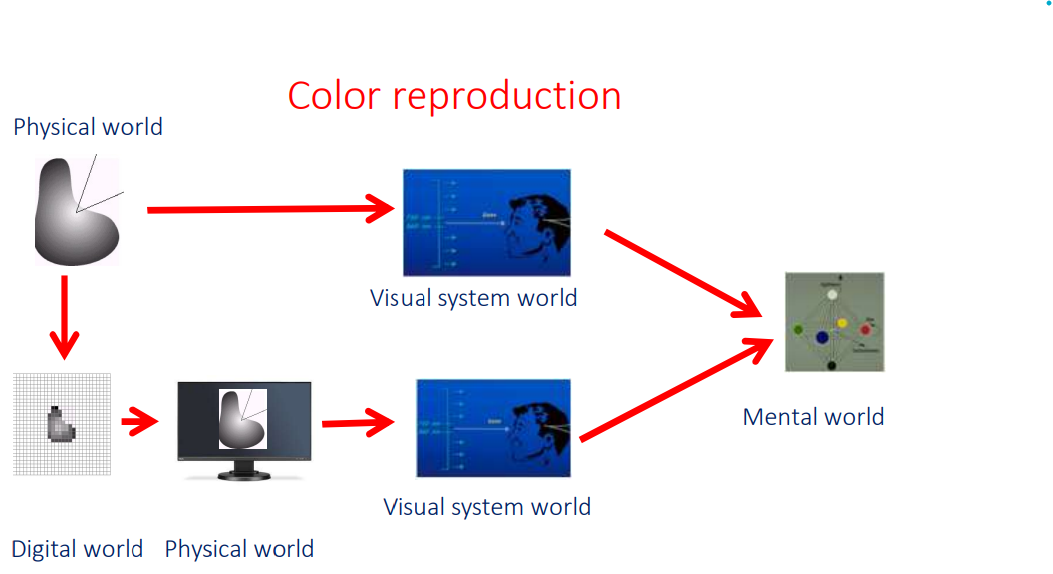
\includegraphics[width=0.5\textwidth]{img/descrizione_colore.png}
    \caption{Diversi punti di vista}
    \label{fig:significato_colore}
\end{figure}

Quando si vuole riprodurre il colore di un oggetto in modo da digitalizzarlo,
bisogna aggiustare il suo colore in modo che il prodotto visualizzato sullo
schermo sia il più simile possibile all'oggetto reale.
Questa operazione non è così semplice, perché il colore reale è influenzato da
molti fattori. Possiamo dunque introdurre la seguente tassonomia:
\begin{itemize}
    \item \textbf{Pleasing color reproduction}: si riferisce allo sforzo di
          aggiustare il colore in modo che l'utente riconosca l'immagine
          accettabile o realistica.

          In sostanza l'immagine deve essere plausibile, la certezza la si ha
          solo quando si è stati nello stesso posto nello stesso giorno.
    \item \textbf{Colorimetric color reproduction}: si riferisce al rappresentare
          il reale colore dell'oggetto con un ridotto errore.

          In sostanza si cerca di riprodurre il colore originale sotto le stesse
          condizioni di vista e di materiali.
    \item \textbf{Color appearance reproduction}: richiede un modello di color
          appearance, ovvero informazioni sulle condizioni di vista dell'oggetto
          originale e di quello digitale e un'accurata calibrazione e
          caratterizzazione di tutti i device.
    \item \textbf{Color preference reproduction}: manipola i colori dell'immagine
          in modo tale che il risultato sia preferibile agli utenti sotto
          un'accurata riproduzione delle apparenze. Si modifica l'immagine
          togliendo il rumore o regolando i colori.
    \item \textbf{Spectral color reproduction}: effettua un'identica riproduzione
          dello spettro di riflettanza dell'immagine o dell'oggetto originale.
\end{itemize}

Ogni singolo dispositivo ha un proprio processo fisico di gestione dell'immagine
e questo permette al device di utilizzare un proprio spazio colore di lavoro
chiamato \textbf{device dependent color imaging} (RGB, CMY, \dots).

\begin{definizione}[\textbf{Device dependent color space}]
    Formalmente \textbf{device dependent color space} è un modello matematico
    astratto che descrive come i colori devono essere rappresentati mediante le
    tuple.
\end{definizione}

Si utilizzano spazi colori differenti tra i device perché ognuno ha la capacità
di rappresentare una particolare gamma di colori. Si cerca quindi di utilizzare
uno spazio la contenga interamente.

\begin{definizione}[\textbf{Device independent color space}]
    Formalmente \textbf{device independent color space} è uno spazio in cui
    esiste almeno una trasformazione tra device dependent color space e uno
    spazio standard CIE.
\end{definizione}

Se non esiste una trasformazione del genere allora lo spazio colore è device
dependent (DD). Mentre, lo spazio device independent (DI) è anche chiamato
\textbf{un-rendered} dal momento che i valori descrivono la colorimetria.

\begin{nota}
    Ricorda che DD e DI sono anche chiamati assoluto e non assoluto.
\end{nota}

Esistono diversi spazi colore device independent, questi possono essere
convertiti tra di loro mediante delle trasformazioni. Specificare le relazioni
tra i diversi tipi di spazi colore, ovvero tra quelli device dependent e
device independent, è chiamato \textbf{caratterizzazione} del dispositivo.

\section{RGB based Color Management}
In generale, quando acquisiamo un'immagine attraverso un dispositivo, si ottiene
una rappresentazione DD dell'immagine. Ottenuta questa codifica, si sfrutta la
caratterizzazione del dispositivo per ottenere la rappresentazione DI.

Mentre, per quanto riguarda il processo di visualizzazione dell'immagine, si
parte dalla codifica device independent, si applica la caratterizzazione del
dispositivo di output e si ottiene la rappresentazione device independent.

I vantaggi di questo approccio sono:
\begin{itemize}
    \item Ogni applicazione deve solo definire le trasformazioni tra il suo spazio
          colore e gli spazi standard.
    \item Si ha uno standard che evita l'incompatibilità.
\end{itemize}
Lo svantaggio di questa tecnica sono:
\begin{itemize}
    \item Le trasformazioni sono necessarie per lo scambio delle immagini.
    \item La maggior parte del software si deve modificare.
\end{itemize}

Si potrebbe pensare di utilizzare direttamente uno standard device independent.
Il problema è che non è fisicamente possibile creare dei dispositivi che
rappresentino quello specifico spazio colore o sarebbe troppo costoso.
Perciò, si utilizzano delle varianti per permetterci di ridurre lo spazio
utilizzato.

Le rappresentazioni device dependent hanno delle conversioni tra di loro,
l'importante è che si preservino gli stessi colori. Gli altri spazi colori sono
generalmente usati per l'image processing tasks.

Le trasformazioni da device independent a device dependent avvengono seguendo i
seguenti passi:
\begin{itemize}
    \item \textbf{Chromatic adaptation transform} (CAT): si modifica l'illuminazione
          per rendere distinguibili gli oggetti nella scena. In sostanza si
          applica una moltiplicazione di matrice che per passare da una luce
          standard della scena alla luce standard del DD.
    \item \textbf{Conversione da DI a DD}: si sfruttano le leggi date dalla
          caratterizzazione del dispositivo per ottenere la rappresentazione
          device dependent.
    \item \textbf{Gamma correction}: si corregge la gamma in modo tale che si
          migliori la visione dei colori dell'immagine rispetto al dispositivo
          di output.
\end{itemize}

Gli spazi device dependent hanno uno standard per semplificare la
caratterizzazione del dispositivo. Infatti, avendo definito degli standard si
ha già la conversione da DI a DD e viceversa.
\begin{nota}
    Gli spazi standard sono anche detti \textbf{rendered space}.
\end{nota}

Per definire uno spazio device dependent standard c'è bisogno di specificare
delle primitive lineari e una reference del punto di bianco. Il problema è che
spesso le primitive non sono lineari a causa di una gamma correction. Quindi, si
aggiungono parametri per modellare questa non linearità.

\begin{nota}
    Per esempio tutti gli spazi basati su RGB necessitano della definizione delle
    primitive, il punto di bianco, il parametro della gamma correction, $s$ che
    determina l'inclinazione della parte lineare, $t$  determina l'inclinazione
    della parte non lineare e $f$ è l'offset.
\end{nota}

Ricorda che quando si effettua la conversione tra gli spazi colori si possono
incorrere in problemi legati alle \textbf{limitazioni della gamma} e questo porta
ad avere modifiche della gamma rappresentabile. Se noi partiamo da uno spazio
$s_1$ e convertiamo ad uno spazio $s_2$ allora i colori rappresentabili diventano
$\gamma(s_1)\cap \gamma(s_2)$ l'intersezione della gamma dei due spazi.

